%-----------------------------------------------------------------------------------------------------------------------------------------------%
%	The MIT License (MIT)
%
%	Copyright (c) 2015 Jan Küster
%
%	Permission is hereby granted, free of charge, to any person obtaining a copy
%	of this software and associated documentation files (the "Software"), to deal
%	in the Software without restriction, including without limitation the rights
%	to use, copy, modify, merge, publish, distribute, sublicense, and/or sell
%	copies of the Software, and to permit persons to whom the Software is
%	furnished to do so, subject to the following conditions:
%	
%	THE SOFTWARE IS PROVIDED "AS IS", WITHOUT WARRANTY OF ANY KIND, EXPRESS OR
%	IMPLIED, INCLUDING BUT NOT LIMITED TO THE WARRANTIES OF MERCHANTABILITY,
%	FITNESS FOR A PARTICULAR PURPOSE AND NONINFRINGEMENT. IN NO EVENT SHALL THE
%	AUTHORS OR COPYRIGHT HOLDERS BE LIABLE FOR ANY CLAIM, DAMAGES OR OTHER
%	LIABILITY, WHETHER IN AN ACTION OF CONTRACT, TORT OR OTHERWISE, ARISING FROM,
%	OUT OF OR IN CONNECTION WITH THE SOFTWARE OR THE USE OR OTHER DEALINGS IN
%	THE SOFTWARE.
%	
%
%-----------------------------------------------------------------------------------------------------------------------------------------------%


%============================================================================%
%
%	DOCUMENT DEFINITION
%
%============================================================================%

%we use article class because we want to fully customize the page and dont use a cv template
\documentclass[10pt,A4]{article}	


%----------------------------------------------------------------------------------------
%	ENCODING
%----------------------------------------------------------------------------------------

%we use utf8 since we want to build from any machine
\usepackage[utf8]{inputenc}		

%----------------------------------------------------------------------------------------
%	LOGIC
%----------------------------------------------------------------------------------------

% provides \isempty test
\usepackage{xifthen}

%----------------------------------------------------------------------------------------
%	FONT
%----------------------------------------------------------------------------------------

% some tex-live fonts - choose your own

%\usepackage[defaultsans]{droidsans}
%\usepackage[default]{comfortaa}
%\usepackage{cmbright}
\usepackage[default]{raleway}
% \usepackage{fetamont}
% \usepackage[default]{gillius}
% \usepackage[light,math]{iwona}
% \usepackage[thin]{roboto} 

% set font default
\renewcommand*\familydefault{\sfdefault} 	
\usepackage[T1]{fontenc}

% more font size definitions
\usepackage{moresize}		

\usepackage{fontawesome}

%----------------------------------------------------------------------------------------
%	PAGE LAYOUT  DEFINITIONS
%----------------------------------------------------------------------------------------

%debug page outer frames
%\usepackage{showframe}			


%define page styles using geometry
\usepackage[a4paper]{geometry}		

% for example, change the margins to 2 inches all round
\geometry{top=1.75cm, bottom=-.6cm, left=1cm, right=1cm} 	

%use customized header
\usepackage{fancyhdr}				
\pagestyle{fancy}

%less space between header and content
\setlength{\headheight}{-5pt}		


%customize entries left, center and right
\lhead{}
\chead{ \small{Nicholas A. Del Grosso  $\cdot$  Munich, Germany  $\cdot$  \textcolor{sectcol}{\textbf{delgrosso.nick@gmail.com}}  $\cdot$ +49 170 8253289 $\cdot$ \faicon{github} nickdelgrosso}
}
\rhead{}


%indentation is zero
\setlength{\parindent}{0mm}

%Hyphenation penalty
\hyphenpenalty

%----------------------------------------------------------------------------------------
%	TABLE /ARRAY/LIST DEFINITIONS
%---------------------------------------------------------------------------------------- 

%for layouting tables
\usepackage{multicol}			
\usepackage{multirow}

%extended aligning of tabular cells
\usepackage{array}

\newcolumntype{x}[1]{%
>{\raggedleft\hspace{0pt}}p{#1}}%

\usepackage{enumitem}


%----------------------------------------------------------------------------------------
%	GRAPHICS DEFINITIONS
%---------------------------------------------------------------------------------------- 

%for header image
\usepackage{graphicx}

%for floating figures
\usepackage{wrapfig}
\usepackage{float}
%\floatstyle{boxed} 
%\restylefloat{figure}

%for drawing graphics		
\usepackage{tikz}				
\usetikzlibrary{shapes, backgrounds,mindmap, trees}


%----------------------------------------------------------------------------------------
%	Color DEFINITIONS
%---------------------------------------------------------------------------------------- 

\usepackage{color}

%accent color
\definecolor{bgcol}{RGB}{13,82,107}

%dark background color
\definecolor{sectcol}{RGB}{170,80,0}

%light background / accent color
\definecolor{softcol}{RGB}{225,225,225}


%============================================================================%
%
%
%	DEFINITIONS
%
%
%============================================================================%

%----------------------------------------------------------------------------------------
% 	HEADER
%----------------------------------------------------------------------------------------

% remove top header line
\renewcommand{\headrulewidth}{0pt} 

%remove botttom header line
\renewcommand{\footrulewidth}{0pt}	  	

%remove pagenum
\renewcommand{\thepage}{}	

%remove section num		
\renewcommand{\thesection}{}			

%----------------------------------------------------------------------------------------
% 	ARROW GRAPHICS in Tikz
%----------------------------------------------------------------------------------------

% a six pointed arrow poiting to the left
\newcommand{\tzlarrow}{(0,0) -- (0.2,0) -- (0.3,0.2) -- (0.2,0.4) -- (0,0.4) -- (0.1,0.2) -- cycle;}	

% include the left arrow into a tikz picture
% param1: fill color
%
\newcommand{\larrow}[1]
{\begin{tikzpicture}[scale=0.58]
	 \filldraw[fill=#1!100,draw=#1!100!black]  \tzlarrow
 \end{tikzpicture}
}

% a six pointed arrow poiting to the right
\newcommand{\tzrarrow}{ (0,0.2) -- (0.1,0) -- (0.3,0) -- (0.2,0.2) -- (0.3,0.4) -- (0.1,0.4) -- cycle;}

% include the right arrow into a tikz picture
% param1: fill color
%
\newcommand{\rarrow}
{
\begin{tikzpicture}[scale=0.7]
	\filldraw[fill=sectcol!100,draw=sectcol!100!black] \tzrarrow
 \end{tikzpicture}
}



%----------------------------------------------------------------------------------------
%	custom sections
%----------------------------------------------------------------------------------------

% create a coloured box with arrow and title as cv section headline
% param 1: section title
%
\newcommand{\cvsection}[1]
{
\colorbox{bgcol}{\makebox[1\linewidth][l]{
	\larrow{sectcol} \hspace{-8pt} \larrow{sectcol} \hspace{-8pt} \larrow{sectcol} \textcolor{white}{\textbf{#1}}\hspace{4pt}
}}\\
}

%create a coloured arrow with title as cv meta section section
% param 1: meta section title
%
\newcommand{\metasection}[2]{
	\begin{tabular*}{1\linewidth}{p{0.18\linewidth} p{0.76\linewidth}}
		\larrow{bgcol}\normalsize{\textbf{\textcolor{sectcol}{#1}}}&#2\\
	\end{tabular*}
	
    \vspace{3pt}
}

%----------------------------------------------------------------------------------------
%	 CV EVENT
%----------------------------------------------------------------------------------------

% creates a stretched box as cv entry headline followed by two paragraphs about 
% the work you did
% param 1:	event time i.e. 2014 or 2011-2014 etc.
% param 2:	event name (what did you do?)
% param 3:	institution (where did you work / study)
% param 4:	what was your position
% param 5:	some words about your contributions
%
\newcommand{\cvevent}[5] {
\begin{flushleft}
\textcolor{sectcol}{#1,  #3}\\
\textbf{#2}\\[-7pt]
\textcolor{softcol}{\hrule}
\vspace{\spread}
\begin{tabular*}{1\linewidth}{p{0.001\linewidth} p{0.9\linewidth}}
	\larrow{bgcol} & #4 \\[2pt]
	\larrow{bgcol} & #5 \\[\spread]
\end{tabular*}
\end{flushleft}
%\textcolor{softcol}{\hrule}
}

% creates a stretched box as 
\newcommand{\cveventmeta}[2] {
	\mbox{\mystrut \hspace{87pt}\textit{#1}}\\
	#2
}

%----------------------------------------------------------------------------------------
% CUSTOM STRUT FOR EMPTY BOXES
%----------------------------------------- -----------------------------------------------
\newcommand{\mystrut}{\rule[-.3\baselineskip]{0pt}{\baselineskip}}

%----------------------------------------------------------------------------------------
% CUSTOM LOREM IPSUM
%----------------------------------------------------------------------------------------
\newcommand{\lorem}
{Lorem ipsum dolor sit amet, consectetur adipiscing elit. Donec a diam lectus.}

%----------------------------------------------------------------------------------------
% SPREAD
%----------------------------------------------------------------------------------------
\newcommand{\spread}{7pt}

%============================================================================%
%
%
%
%	DOCUMENT CONTENT
%
%
%
%============================================================================%
\begin{document}


%use our custom fancy header definitions
\pagestyle{fancy}



\begin{minipage}[t]{0.485\textwidth}

\vspace{\spread}

%---------------------------------------------------------------------------------------
%	TITLE HEADLINE
%----------------------------------------------------------------------------------------

\hspace{-0.15\linewidth}\colorbox{bgcol}{\makebox[1.15\linewidth][c]{\textcolor{sectcol}{\rule[-1mm]{1mm}{0.9cm}} \Huge{\textcolor{white}{\textsc{Nicholas}} } \Huge{\textcolor{white}{\textsc{Del Grosso}} } }}

%----------------------------------------------------------------------------------------
%	HEADER IMAGE
%----------------------------------------------------------------------------------------
\hspace{-0.25\linewidth}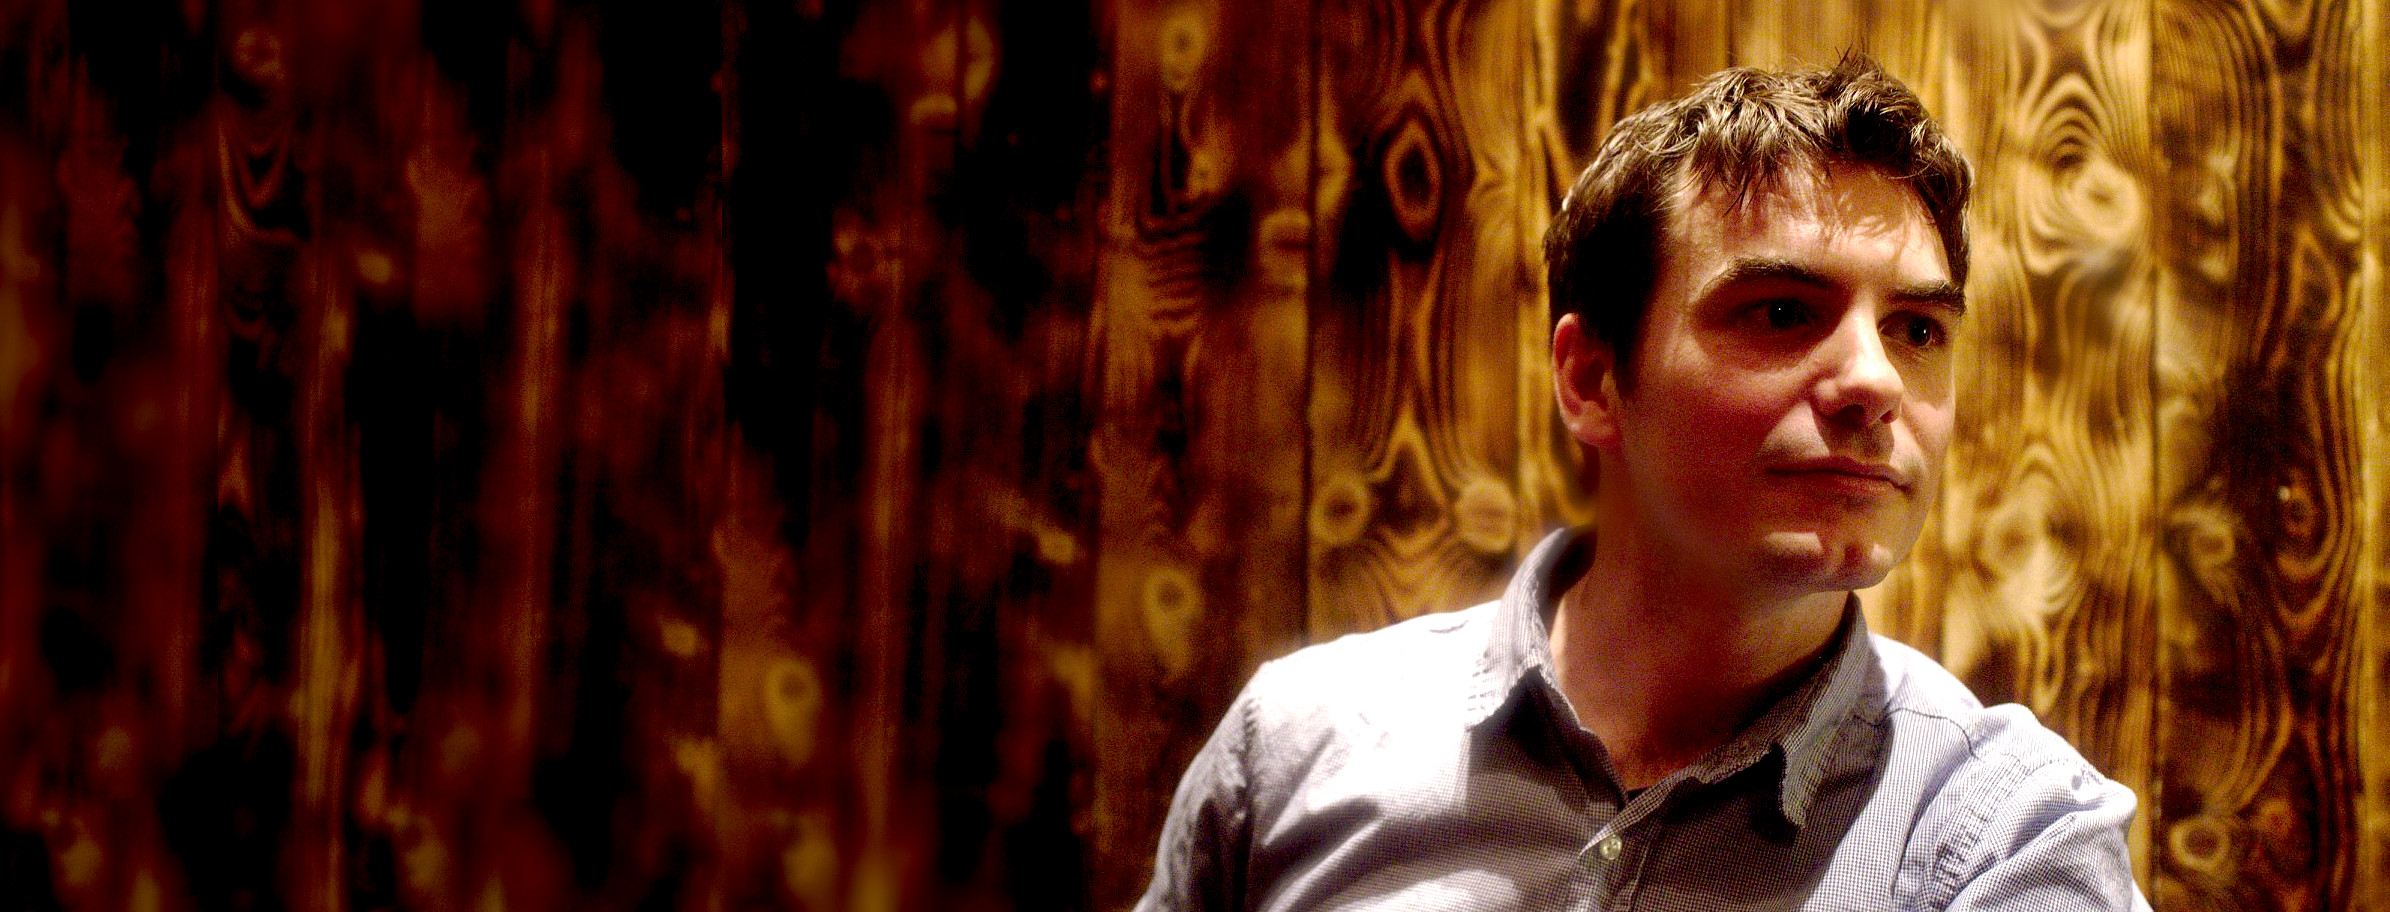
\includegraphics[width=1.2725\linewidth, height=4.4cm]{../my_foto.jpg} %use full size

%---------------------------------------------------------------------------------------
%	QR CODE (optional)
%----------------------------------------------------------------------------------------
% \vspace{-100pt}
% \hspace{0.59\linewidth}
% \includegraphics[width=88pt]{qrcode}
% \normalsize


\vspace{5pt}

\end{minipage} 
\hfill
\begin{minipage}[t]{0.485\textwidth}
%---------------------------------------------------------------------------------------
%	SUMMARY (optional)
%----------------------------------------------------------------------------------------
\vspace{\spread}

\cvsection{Zusammenfassung}\\
Ich bin promovierter Neurowissenschaftler mit 10 Jahren Projekterfahrung in wissenschaftlicher Softwareentwicklung und Datenanalyse in Python und R.

\vspace{5pt}

Ich entwickle Ausbildungsprogramme für Wissenschaftler in Datenanalyse und Software-Engineering und unterrichte Methoden aus den Bereichen Software Craftsmanship und Lean Management.  Ich berate auch über wissenschaftliche Open-Source-Software.  Seit ich vor 9 Jahren mit dem Unterrichten begann, habe ich mehr als 500 Wissenschaftlern und Ingenieuren geholfen, ihre Programmierkenntnisse zu verbessern.\\[-2pt]

\end{minipage}

\begin{minipage}[t]{0.485\textwidth}

\vspace{\spread}

%---------------------------------------------------------------------------------------
%	META SECTION
%----------------------------------------------------------------------------------------

\cvsection{Erfahrungen}

\metasection{Data:}{Python, R, Pandas, Numpy, Xarray, Scikit-Learn, PyMC3, Flask, Snakemake, Seaborn, Altair, DVC, HDF5, NetCDF, Jupyter Lab, Papermill, Matlab, SPSS}

\metasection{Tech:}{Git, GitHub, Bash, Linux, Docker, Travis CI, OpenGL, Javascript, Hugo, Netlify, Bootstrap, Trello, PyCharm, VSCode, Blender3D, Adobe Suite}


\metasection{Lehren:}{Python Programming, Statistics in R, Software Engineering, Reseach Project Management, Public Speaking}

\metasection{Sprach:}{Englisch (Muttersprache), Deutsch (B1)}

\metasection{Spass:}{Rätsel, Lesen, Reisen, Design, Mob Programmieren, Hackathons, Science Slams}


\end{minipage}
\hfill
\begin{minipage}[t]{0.485\textwidth}

\vspace{\spread}

\cvsection{Aktueller Status}

\cvevent{July 2019 - Derzeitig}{Freiberuflicher Trainer für Datenwissenschaft und Programmierung}{München, Deutschland }{Unterrichtet praktische Workshops für wissenschaftliche Forscher und Ingenieure.}{Über 600 Stunden Lehrerfahrung, für Klassengrößen von 8-150 Studenten.}

\cvevent{May 2020 - Derzeitig}{Freiberuflicher Remote-Software-Berater}{Remote, München, Deutschland }{Verbessere wissenschaftlicher Open-Source-Software für Kunden im In- und Ausland.}{Profilieren von Algorithmen für Geschwindigkeit, Speichernutzung und IO.}
%

\end{minipage}

\begin{minipage}[t]{0.485\textwidth}

\vspace{\spread}

%---------------------------------------------------------------------------------------
%	EDUCATION SECTION
%--------------------------------------------------------------------------------------

\cvsection{Bildung}

\cvevent{2012-2018}{Ph.D - Systeme Neurowissenschaft}{LMU München}{Entwickelte und baute ein Open-Source VR-System für die Tierverhaltensforschung in Python.}{Unterrichtete Universitätskurse in Python-Programmierung und betreute fünf Studenten in Ingenieur-, Forschungs- und Programmierprojekten mit einer Dauer von 3-12 Monaten.}

%\textcolor{softcol}{\hrule}

%
\cvevent{2010-2012}{M.Sc. - Neurowissenschaft}{Üniversität Tübingen}{Analysierte spektrale und zeitserielle Hirnbildgebungsdaten zur Beurteilung der klinischen Effekte von Physiotherapie und Brain-Machine-Interface-Therapie bei Schlaganfallpatienten}{Organisierte eine studentische Vortragsreihe zur Datenanalyse und implementierte ein Wiki für das Forschungsinstitut.}

%\textcolor{softcol}{\hrule}

%
\cvevent{2006-2010}{B.Sc. - Psychologie}{Wittenberg University, Ohio, USA}{Bau eines NI-DAQ EEG-Systems, programmierte Online-Analyse in Matlab und LabView.}{Lehrassistent für Neurophysiologie (Neurochirurgie bei Nagetieren und Elektrophysiologie).}

%
% \cvevent{2008 - 2009}{Summer Lab Rotations}{Duke University, North Carolina, USA}{Routine electrical engineering (impedence measurements, cable repair) and data analysis (Matlab).}{Animal training for cognitive experiments}


%\textcolor{softcol}{\hrule}

\end{minipage}
\hfill
\begin{minipage}[t]{0.485\textwidth}

\vspace{\spread}

%---------------------------------------------------------------------------------------
%	EXPERIENCE
%----------------------------------------------------------------------------------------
\cvsection{Einschlägige Erfahrung}

\cvevent{Nov. 2019 - March 2020}{Scientific Employee / Workshop Planner}{G-Node, LMU München}{Für die NFDI-Initiative zur Ausbildung in der Computerinfrastruktur entwarf ich einen Kurslehrplan "Forschungsdatenmanagement".}{I Praktische Übungen zu Git und wissenschaftlicher Transparenz vorbereitet.}
%
\cvevent{Nov. 2018 - July 2019}{Coach für Softwaretechnik}{Max Planck Institute für Biochemie, München}{Ich schulte und betreute Forscher in der Python-Datenanalyse an den Standorten München und Kopenhagen der Abteilung.}{Ich integrierte Lean-Managementmethoden in Massenspektrometrie-Workflows durch eine kundenspezifische Anwendung zur Auftragsplanung.}

\cvevent{2014-Present}{Freiwilliger Organisator und Ausbilder von Meetups}{PyData, LMU München, & ReDI Schule}{Organisierte über 70 öffentliche Anleitungsveranstaltungen in Technologieunternehmen für die lokale Datenwissenschaftsgemeinschaft.}{Ich coachte Gastredner für Veranstaltungen (50-200 Teilnehmer), rekrutierte Führungsteams für etablierte Gruppen und unterrichtete Online-Kurse.}

\end{minipage}

%-------------------------------------------------------------------------------------------------
%	ARTIFICIAL FOOTER (fancy footer cannot exceed linewidth) 
%--------------------------------------------------------------------------------------------------

\null
\vspace*{\fill}
\hspace{-0.25\linewidth}\colorbox{white}{\makebox[1.5\linewidth][c]{\mystrut  \textcolor{white}{https://www.linkedin.com/in/nick-del-grosso/} $\cdot$ \textcolor{white}{https://www.github.com/nickdelgrosso}}}




%============================================================================%
%
%
%
%	DOCUMENT END
%
%
%
%============================================================================%
\end{document}
